% Píše: aplikace. Přílohy k aplikaci, každá jako \chapter{...}.
\chapter{Snímky obrazovek aplikace}
\label{chap:app-snimky}

Snímky vznikly automatickými testy obrazovek (oddíl~\ref{sec:testovani-aplikace}) s~ukázkovými
daty: Raspberry Pi hlásí 20.~10.~2026 v~10:00, je den a~termostat je v~režimu Auto. Telefon je
široký 384~dp, tablet na šířku má 1280~$\times$~800~dp. Snímky telefonu na této straně ukazují
celou obrazovku až po konec obsahu.

\begin{figure}[H]
\centering
\begin{minipage}[t]{0.31\textwidth}
  \centering
  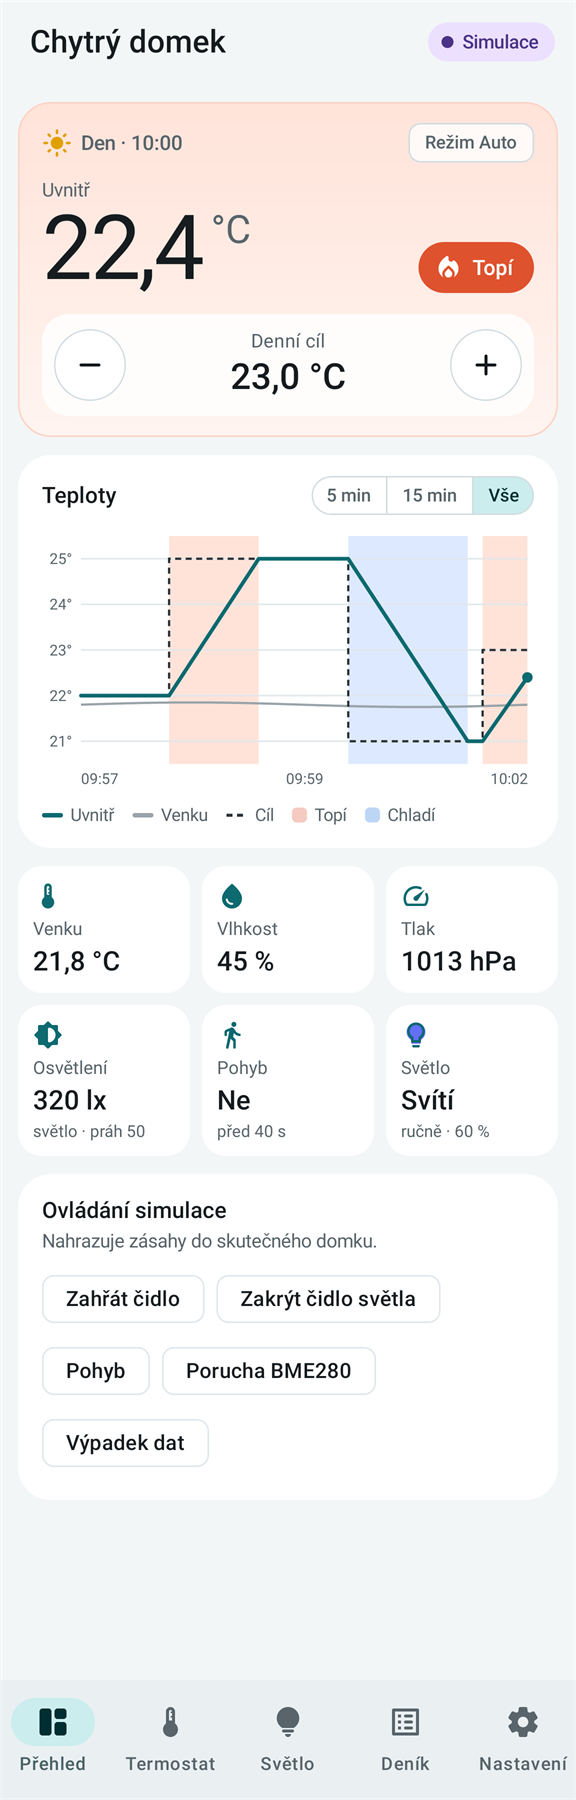
\includegraphics[width=\linewidth]{Figures/aplikace/simulace.png}
  \caption{Přehled v~simulaci s~ovládáním simulace}
  \label{fig:app-simulace}
\end{minipage}\hfill
\begin{minipage}[t]{0.31\textwidth}
  \centering
  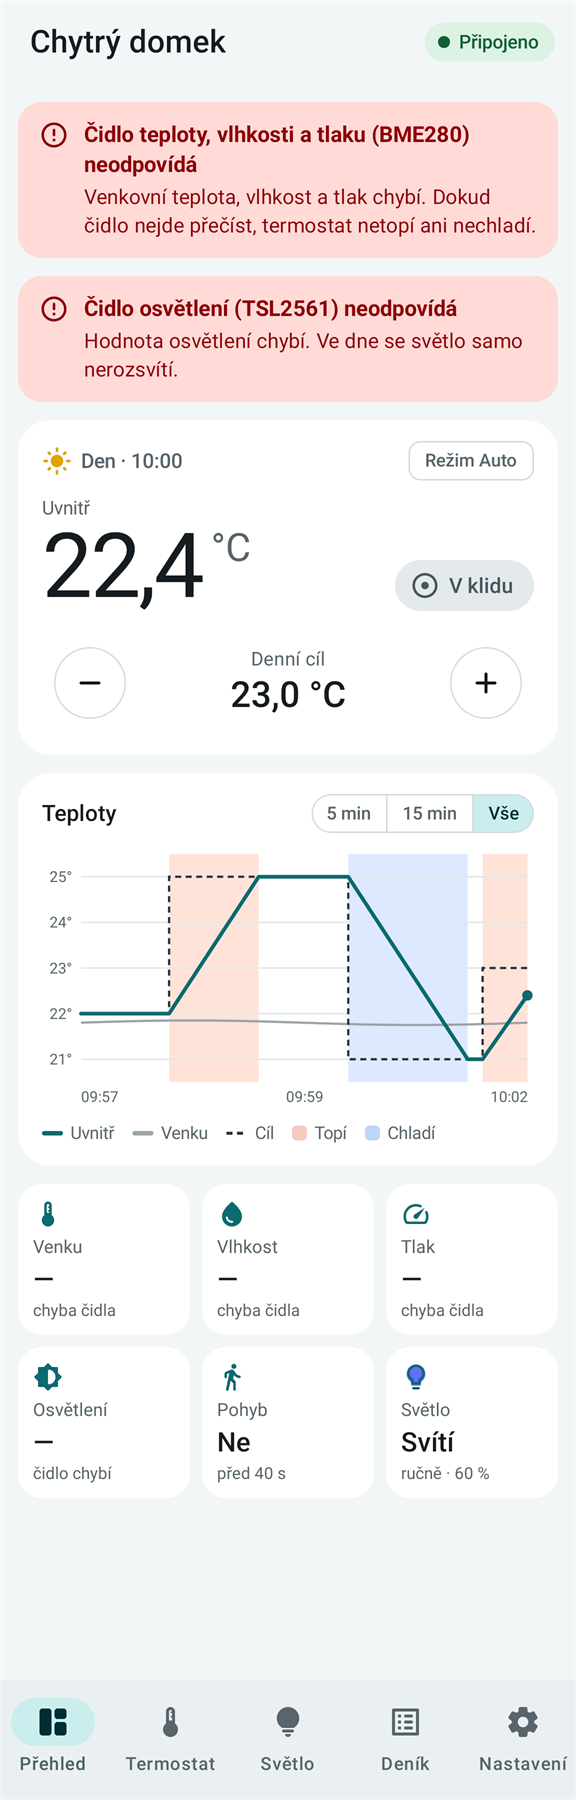
\includegraphics[width=\linewidth]{Figures/aplikace/poruchy-cidel.png}
  \caption{Poruchy obou čidel}
  \label{fig:app-poruchy}
\end{minipage}\hfill
\begin{minipage}[t]{0.31\textwidth}
  \centering
  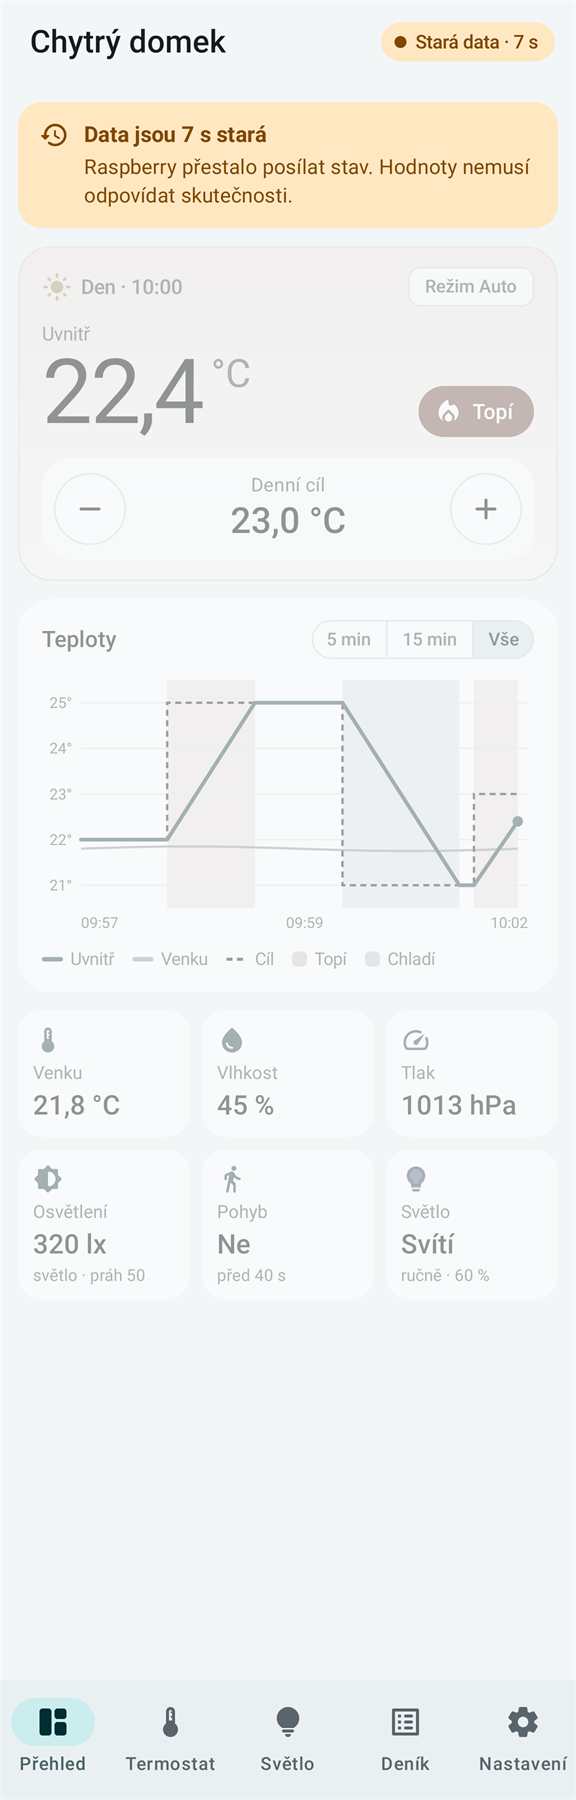
\includegraphics[width=\linewidth]{Figures/aplikace/stara-data.png}
  \caption{Stará data}
  \label{fig:app-stara-data}
\end{minipage}
\end{figure}

\begin{figure}[H]
\centering
\begin{minipage}[t]{0.31\textwidth}
  \centering
  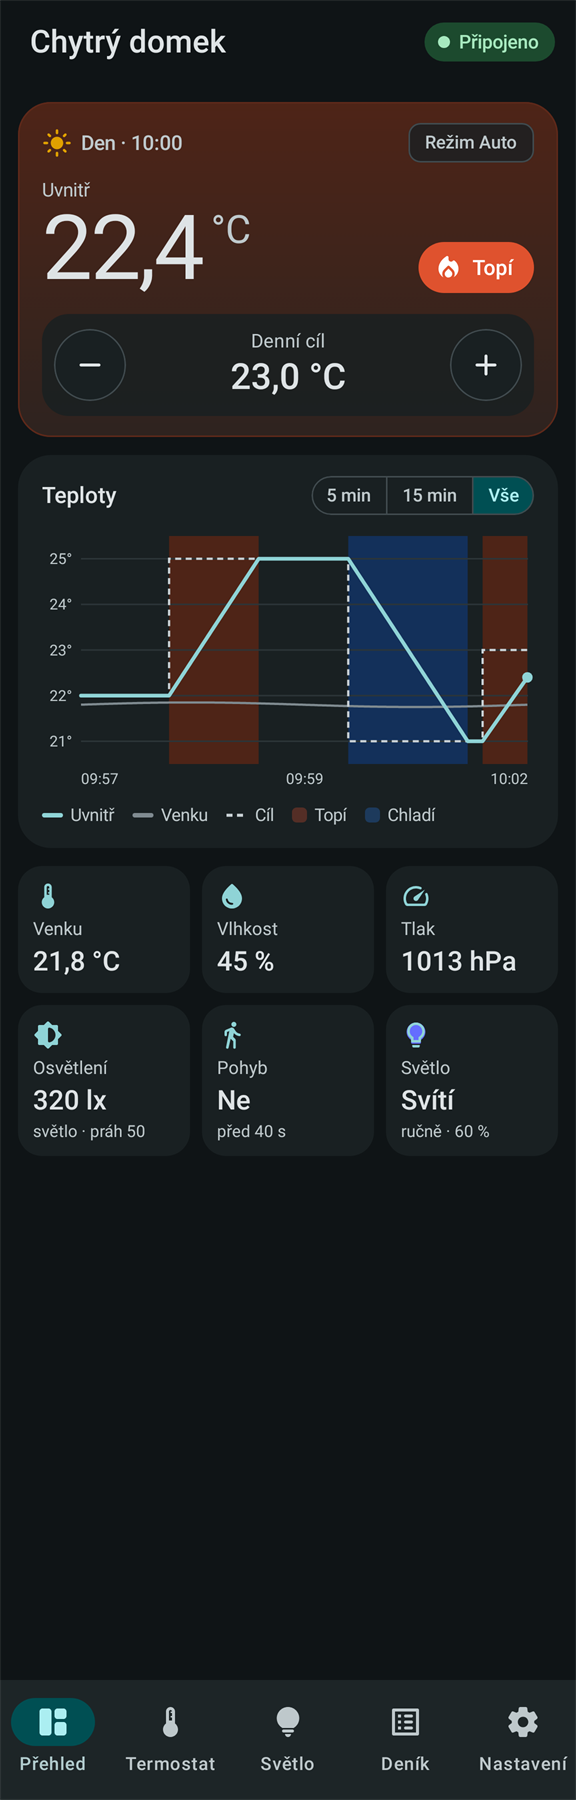
\includegraphics[width=\linewidth]{Figures/aplikace/tmavy-motiv.png}
  \caption{Tmavý motiv}
  \label{fig:app-tmavy-motiv}
\end{minipage}\hspace{0.08\textwidth}%
\begin{minipage}[t]{0.31\textwidth}
  \centering
  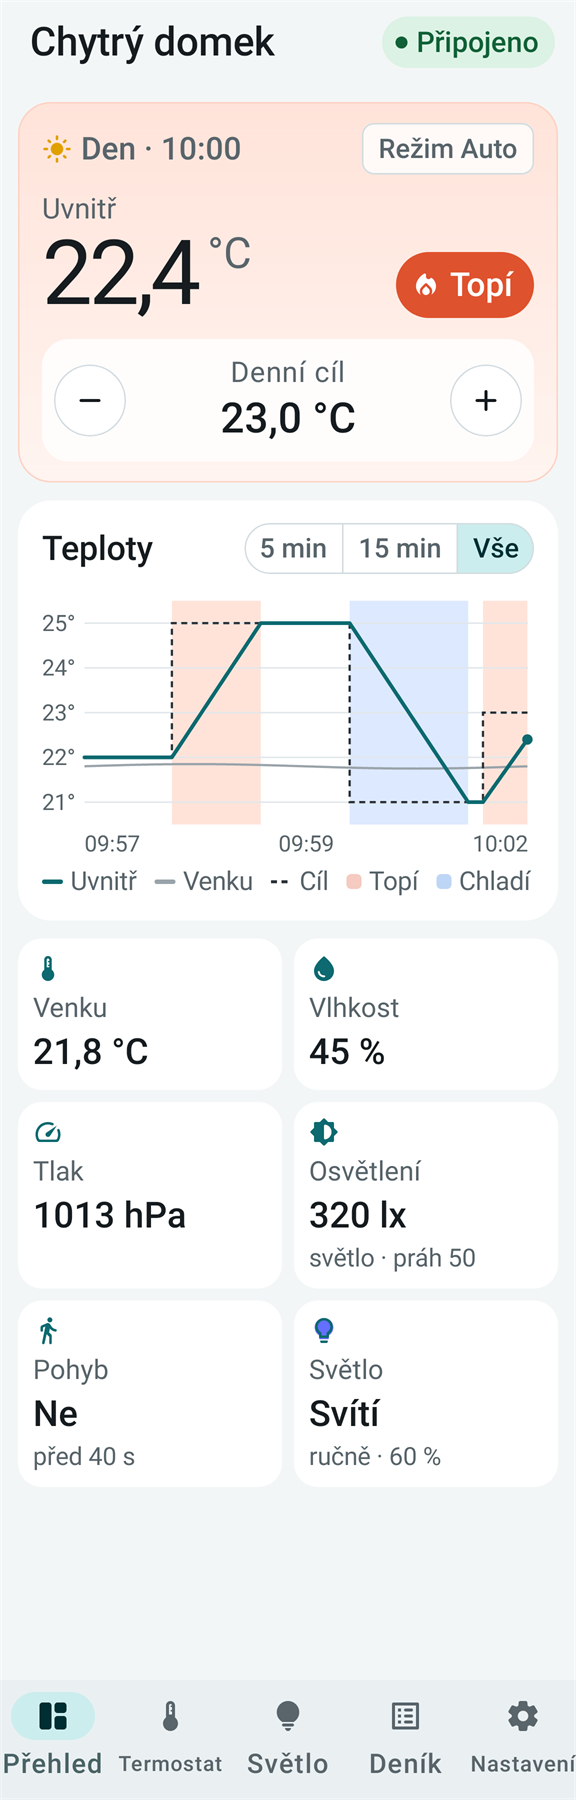
\includegraphics[width=\linewidth]{Figures/aplikace/velke-pismo.png}
  \caption{Písmo zvětšené na 150~\%}
  \label{fig:app-velke-pismo}
\end{minipage}
\end{figure}

\begin{figure}[H]
\centering
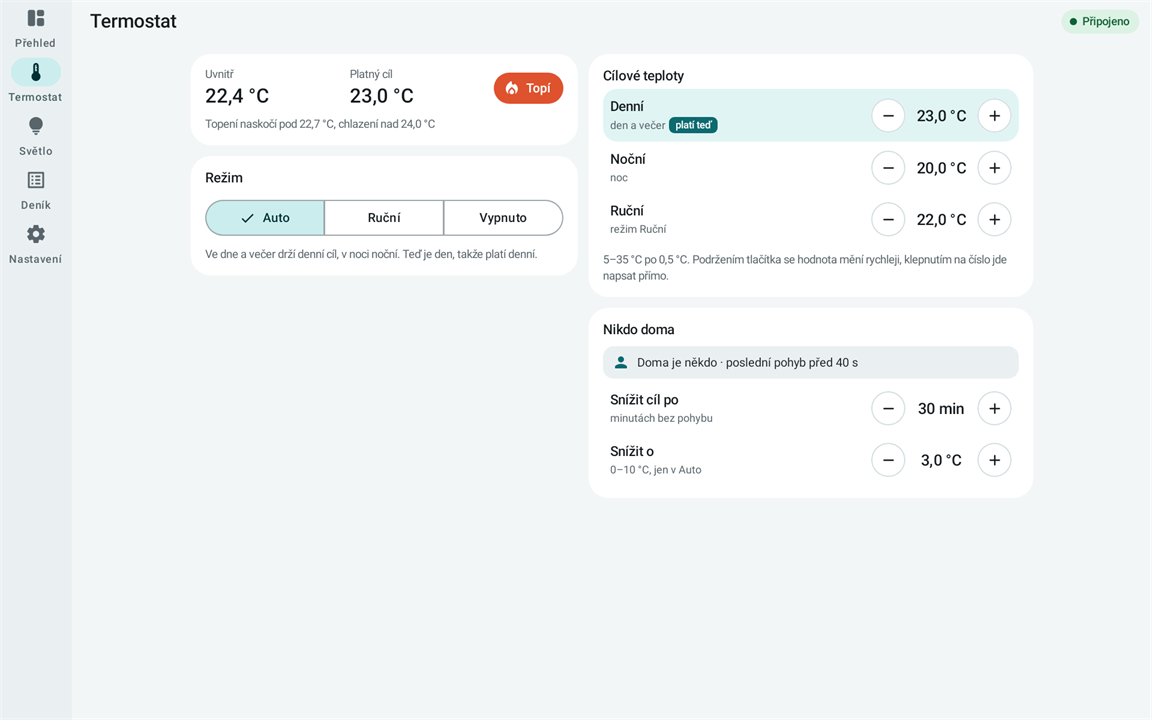
\includegraphics[width=0.9\textwidth]{Figures/aplikace/tablet-termostat.png}
\caption{Termostat na tabletu}
\label{fig:app-tablet-termostat}
\end{figure}

\begin{figure}[H]
\centering
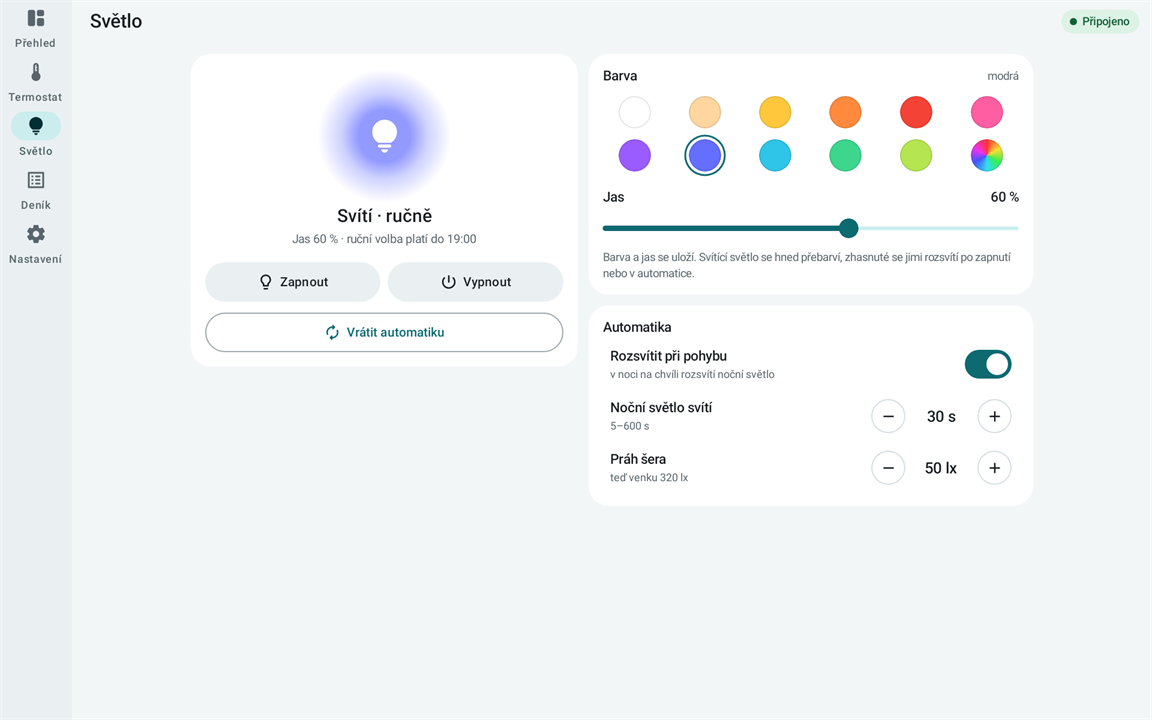
\includegraphics[width=0.9\textwidth]{Figures/aplikace/tablet-svetlo.png}
\caption{Světlo na tabletu}
\label{fig:app-tablet-svetlo}
\end{figure}

\begin{figure}[H]
\centering
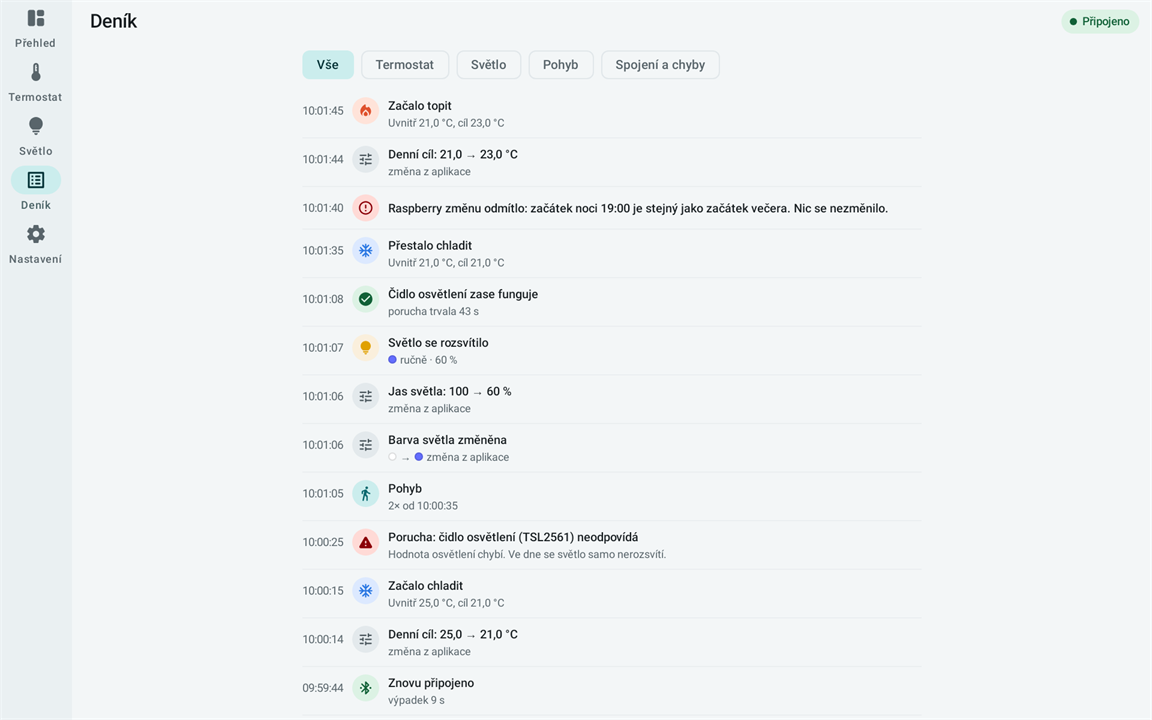
\includegraphics[width=0.9\textwidth]{Figures/aplikace/tablet-denik.png}
\caption{Deník na tabletu}
\label{fig:app-tablet-denik}
\end{figure}

\begin{figure}[H]
\centering
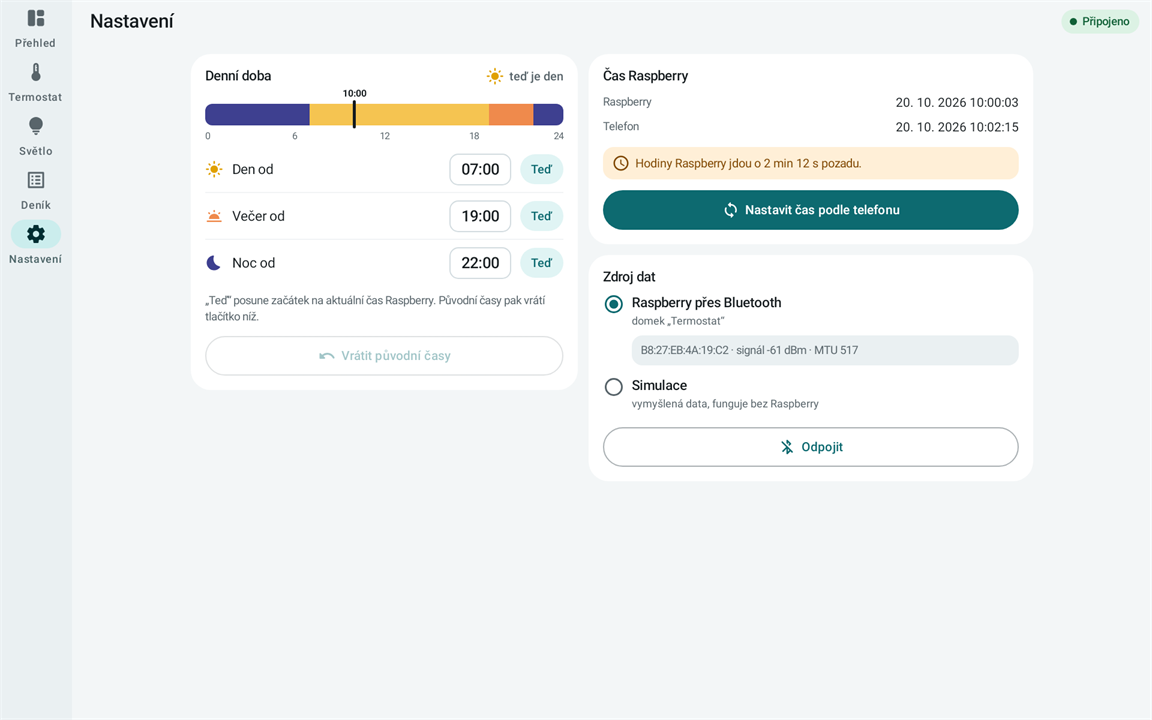
\includegraphics[width=0.9\textwidth]{Figures/aplikace/tablet-nastaveni.png}
\caption{Nastavení na tabletu}
\label{fig:app-tablet-nastaveni}
\end{figure}
